% ------------------------------------------------------------------------------
% Este fichero es parte de la plantilla LaTeX para la realización de Proyectos
% Final de Grado, protegido bajo los términos de la licencia GFDL.
% Para más información, la licencia completa viene incluida en el
% fichero fdl-1.3.tex

% Copyright (C) 2012 SPI-FM. Universidad de Cádiz
% ------------------------------------------------------------------------------


\section{Metodología de desarrollo}
Definición del proceso de desarrollo, ciclo de vida y metodología empleada durante la elaboración del proyecto. Las fases y/o iteraciones que proponga el método empleado deberán quedar recogidas en la planificación que se detalle más adelante.

Se ha optado por una metodología de desarrollo en cascada, como se aprecia en la siguiente imagen:

\begin{figure}[h!]
	\centering
	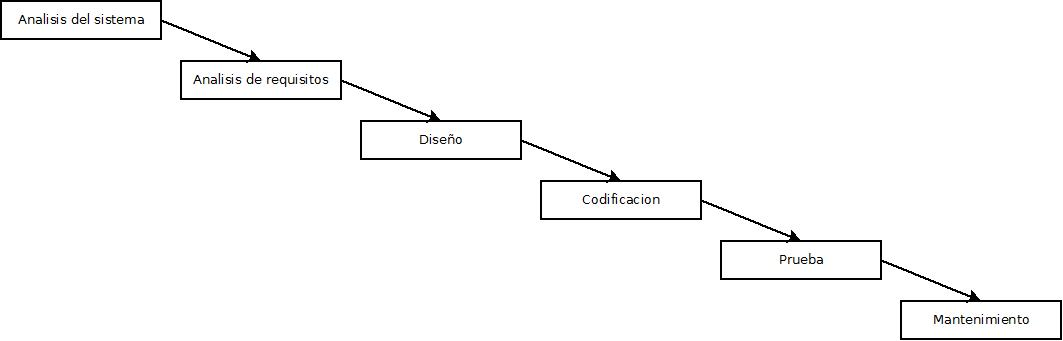
\includegraphics[width=1.0\textwidth]{Cascada.jpg}
	\caption{Desarrollo en cascada.}
\end{figure}

\section{Planificación del proyecto}
Estimación temporal y definición del calendario básico (hitos principales e iteraciones). Desarrollo de la planificación detallada, utilizando un diagrama de Gantt.\\

Se debe incluir una comparación cuantitativa del tiempo y el esfuerzo realmente invertido frente al estimado y planificado. Estos datos pueden recogerse del sistema de gestión de tareas empleado para el seguimiento del proyecto.


\begin{figure}[h]
	\centering
	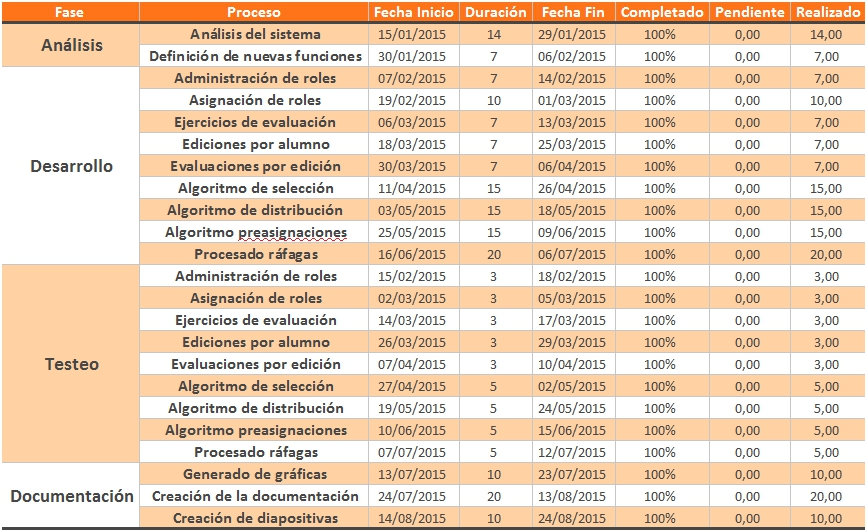
\includegraphics[width=1.0\textwidth]{Gantt-numerico.jpg}
	\caption{Datos del diagrama de Gantt.}
\end{figure}

\begin{figure}[h!]
	\centering
	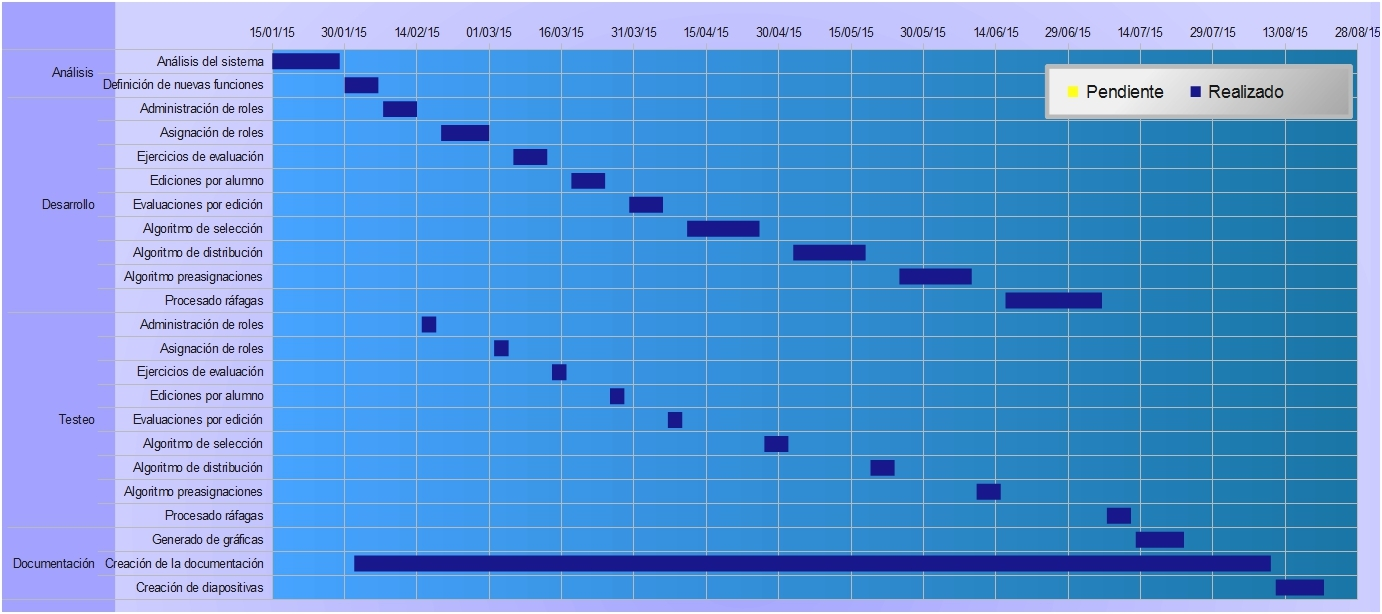
\includegraphics[width=1.0\textwidth]{Gantt-grafica.jpg}
	\caption{Diagrama de Gantt.}
\end{figure}


\begin{figure}[h!]
	\centering
	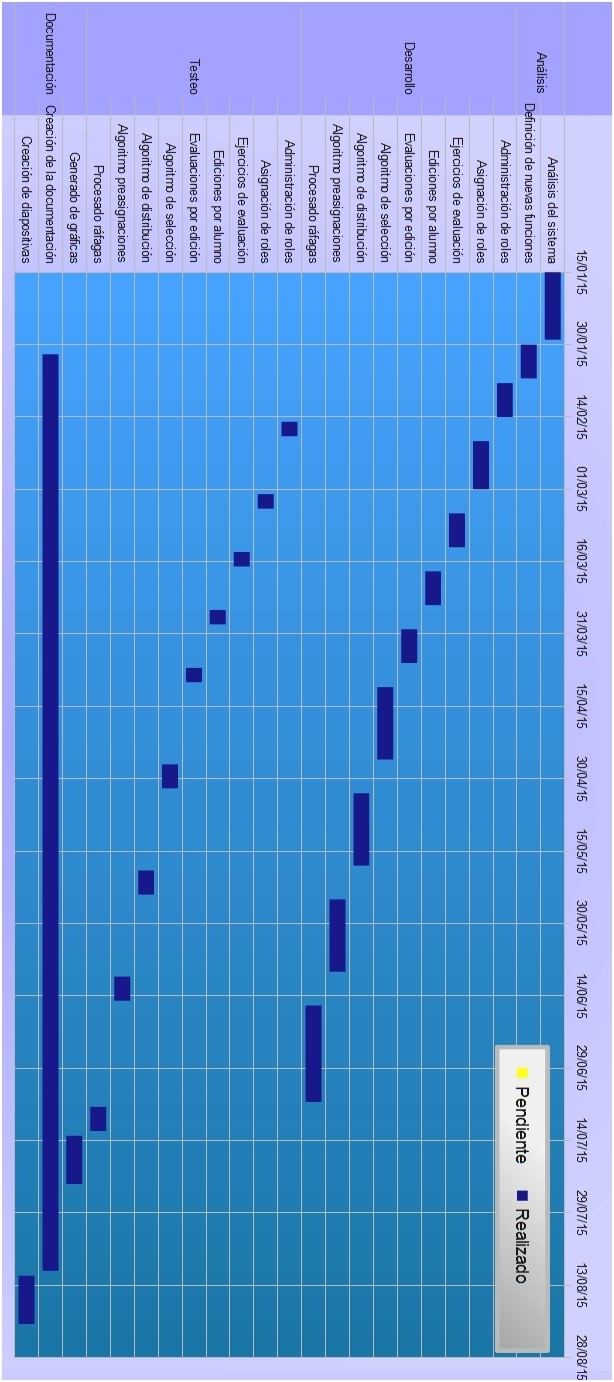
\includegraphics[width=0.6\textwidth]{Gantt-grafica-girada.jpg}
	\caption{Diagrama de Gantt (girada).}
\end{figure}

\clearpage

\section{Organización}
Relación de las personas (roles) involucradas en el proyecto y de cómo se estructuran las relaciones entre las mismas para ejecutar el proyecto. Relación de los recursos inventariables utilizados en el proyecto: equipamiento informático (hardware y software), herramientas empleadas, etc. \\

Para llevar a cabo este proyecto es necesario un MediaWiki. un servidor para alojar AssessMediaWiki y en caso de que el profesor no posea los conocimientos necesarios para la instalación, la colaboración de personal que facilite la instalación de AssessMediaWiki

\section{Riesgos}
Enumeración de los riesgos del proyecto, indicando su posible impacto (efecto que la ocurrencia del citado riesgo tendría en el desarrollo del proyecto) y la probabilidad de ocurrencia. Una vez los riesgos son identificados y priorizados, hay que definir los planes necesarios para reducir los efectos del riesgo una vez se haya materializado o disminuir que este ocurra.\\

De momento hay un pequeño problema con los nombres de los roles creados en el sistema AssessMediaWiki y los ejercicios de evaluación, si los nombres llevan espacio no se podrán eliminar, y es posible que no puedan ser modificados, es un pequeño detalle que se puede arreglar en un trabajo futuro, para evitar este problema basta con usar barras bajas en lugar de espacios.\\

También puede considerarse un riesgo usar el framework (\href{http://www.codeigniter.com/}{CodeIgniter}) sin conocimiento previo, así como que en un futuro dicho framework deje de recibir soporte.
